\documentclass[border=5pt]{standalone}
\usepackage{tikz}
\usetikzlibrary{shapes.geometric, arrows.meta, positioning, fit, backgrounds, calc}
\usepackage{amsmath}

\begin{document}
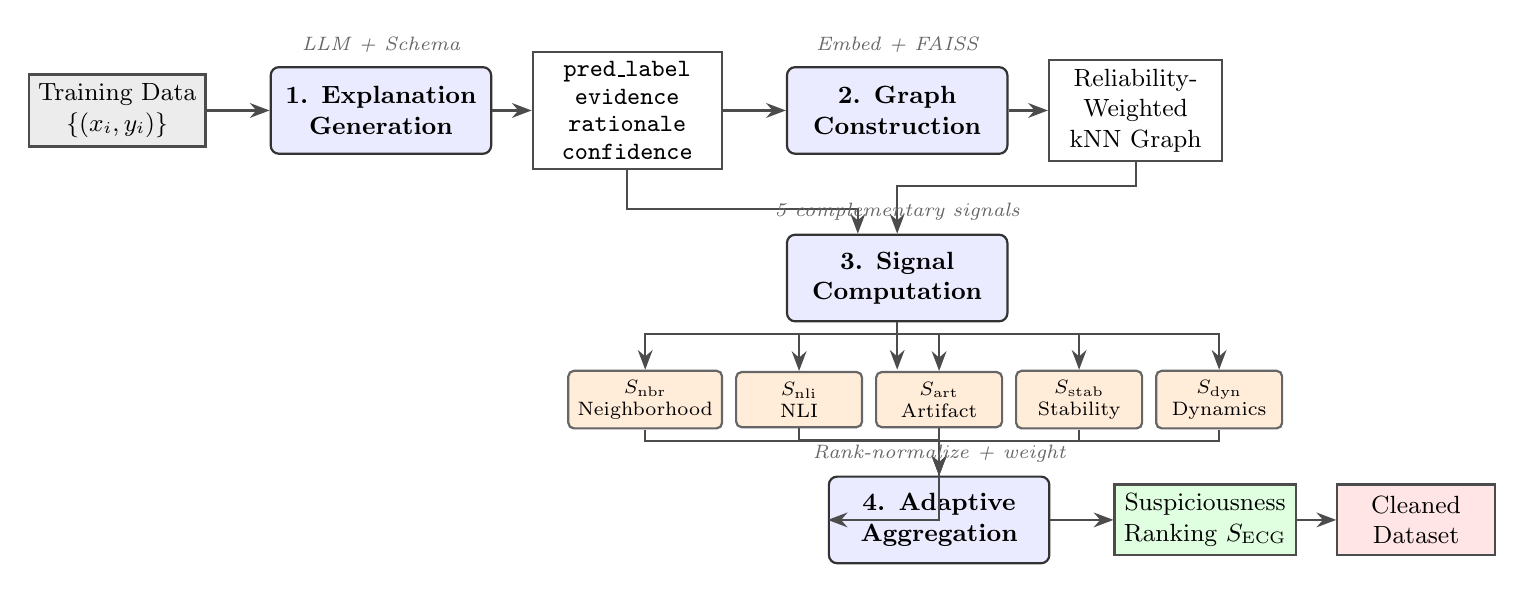
\begin{tikzpicture}[
    node distance=0.4cm and 0.6cm,
    box/.style={rectangle, draw=black!70, fill=white, thick, minimum height=0.9cm, minimum width=2.0cm, align=center, font=\small},
    stage/.style={rectangle, rounded corners=3pt, draw=black!80, fill=blue!8, thick, minimum height=1.1cm, minimum width=2.8cm, align=center, font=\small\bfseries},
    signal/.style={rectangle, rounded corners=2pt, draw=black!60, fill=orange!15, thick, minimum height=0.7cm, minimum width=1.6cm, align=center, font=\scriptsize},
    arrow/.style={-{Stealth[length=2.5mm]}, thick, black!70},
    label/.style={font=\scriptsize\itshape, text=black!60}
]

% Stage 1: Input
\node[box, fill=gray!15] (data) {Training Data\\$\{(x_i, y_i)\}$};

% Stage 2: Explanation Generation
\node[stage, right=0.8cm of data] (explain) {1. Explanation\\Generation};
\node[box, right=0.5cm of explain, minimum width=2.4cm] (json) {\texttt{pred\_label}\\[-1pt]\texttt{evidence}\\[-1pt]\texttt{rationale}\\[-1pt]\texttt{confidence}};

% Stage 3: Graph Construction
\node[stage, right=0.8cm of json] (graph) {2. Graph\\Construction};
\node[box, right=0.5cm of graph, minimum width=2.2cm] (knn) {Reliability-\\Weighted\\kNN Graph};

% Stage 4: Signals
\node[stage, below=1.0cm of graph] (signals) {3. Signal\\Computation};

% Individual signals
\node[signal, below=0.6cm of signals, xshift=-3.2cm] (snbr) {$S_{\text{nbr}}$\\Neighborhood};
\node[signal, right=0.15cm of snbr] (snli) {$S_{\text{nli}}$\\NLI};
\node[signal, right=0.15cm of snli] (sart) {$S_{\text{art}}$\\Artifact};
\node[signal, right=0.15cm of sart] (sstab) {$S_{\text{stab}}$\\Stability};
\node[signal, right=0.15cm of sstab] (sdyn) {$S_{\text{dyn}}$\\Dynamics};

% Stage 5: Aggregation
\node[stage, below=0.6cm of sart] (agg) {4. Adaptive\\Aggregation};

% Output
\node[box, right=0.8cm of agg, fill=green!12] (output) {Suspiciousness\\Ranking $S_{\text{ECG}}$};
\node[box, right=0.5cm of output, fill=red!10] (clean) {Cleaned\\Dataset};

% Arrows
\draw[arrow] (data) -- (explain);
\draw[arrow] (explain) -- (json);
\draw[arrow] (json) -- (graph);
\draw[arrow] (graph) -- (knn);
\draw[arrow] (knn.south) -- ++(0,-0.3) -| (signals.north);
\draw[arrow] (json.south) -- ++(0,-0.5) -| ([xshift=-0.5cm]signals.north);

\draw[arrow] (signals) -- (snbr.north -| signals);
\draw[arrow] (signals.south) -- ++(0,-0.15) -| (snbr.north);
\draw[arrow] (signals.south) -- ++(0,-0.15) -| (snli.north);
\draw[arrow] (signals.south) -- ++(0,-0.15) -| (sart.north);
\draw[arrow] (signals.south) -- ++(0,-0.15) -| (sstab.north);
\draw[arrow] (signals.south) -- ++(0,-0.15) -| (sdyn.north);

\draw[arrow] (snbr.south) -- ++(0,-0.15) -| (agg.north);
\draw[arrow] (snli.south) -- ++(0,-0.15) -| (agg.north);
\draw[arrow] (sart.south) |- (agg.west);
\draw[arrow] (sstab.south) -- ++(0,-0.15) -| (agg.north);
\draw[arrow] (sdyn.south) -- ++(0,-0.15) -| (agg.north);

\draw[arrow] (agg) -- (output);
\draw[arrow] (output) -- (clean);

% Labels
\node[label, above=0.05cm of explain] {LLM + Schema};
\node[label, above=0.05cm of graph] {Embed + FAISS};
\node[label, above=0.05cm of signals] {5 complementary signals};
\node[label, above=0.05cm of agg] {Rank-normalize + weight};

\end{tikzpicture}
\end{document}

